\section{Grundbegriffe der Wahrscheinlichkeitsrechnung}

\subsection{Eine kurze Geschichte der Wahrscheinlichkeitsrechnung}

Lange Zeit hielt man den Zufall für wahrlich „unberechenbar“ und den Mathematikern kam es nicht in den Sinn, sich damit zu befassen. So dauerte es bis ins 16. Jahrhundert, ehe das erste Buch eines Mathematikers zur Wahrscheinlichkeitsrechnung entstand. Es hiess \textit{Liber de Ludo Aleae} (= Das Buch vom Würfelspiel) und wurde vom italienischen Mathematiker Gerolamo Cardano verfasst. Wann genau das Buch entstanden ist, weiss man allerdings nicht, weil Cardano die Überlegungen erstmals für sich behielt, um seinen Vorteil im Glücksspiel zu bewahren. Das Buch wurde dann erst nach Cardanos Tod veröffentlicht.
\begin{figure}[ht]
\begin{center}
        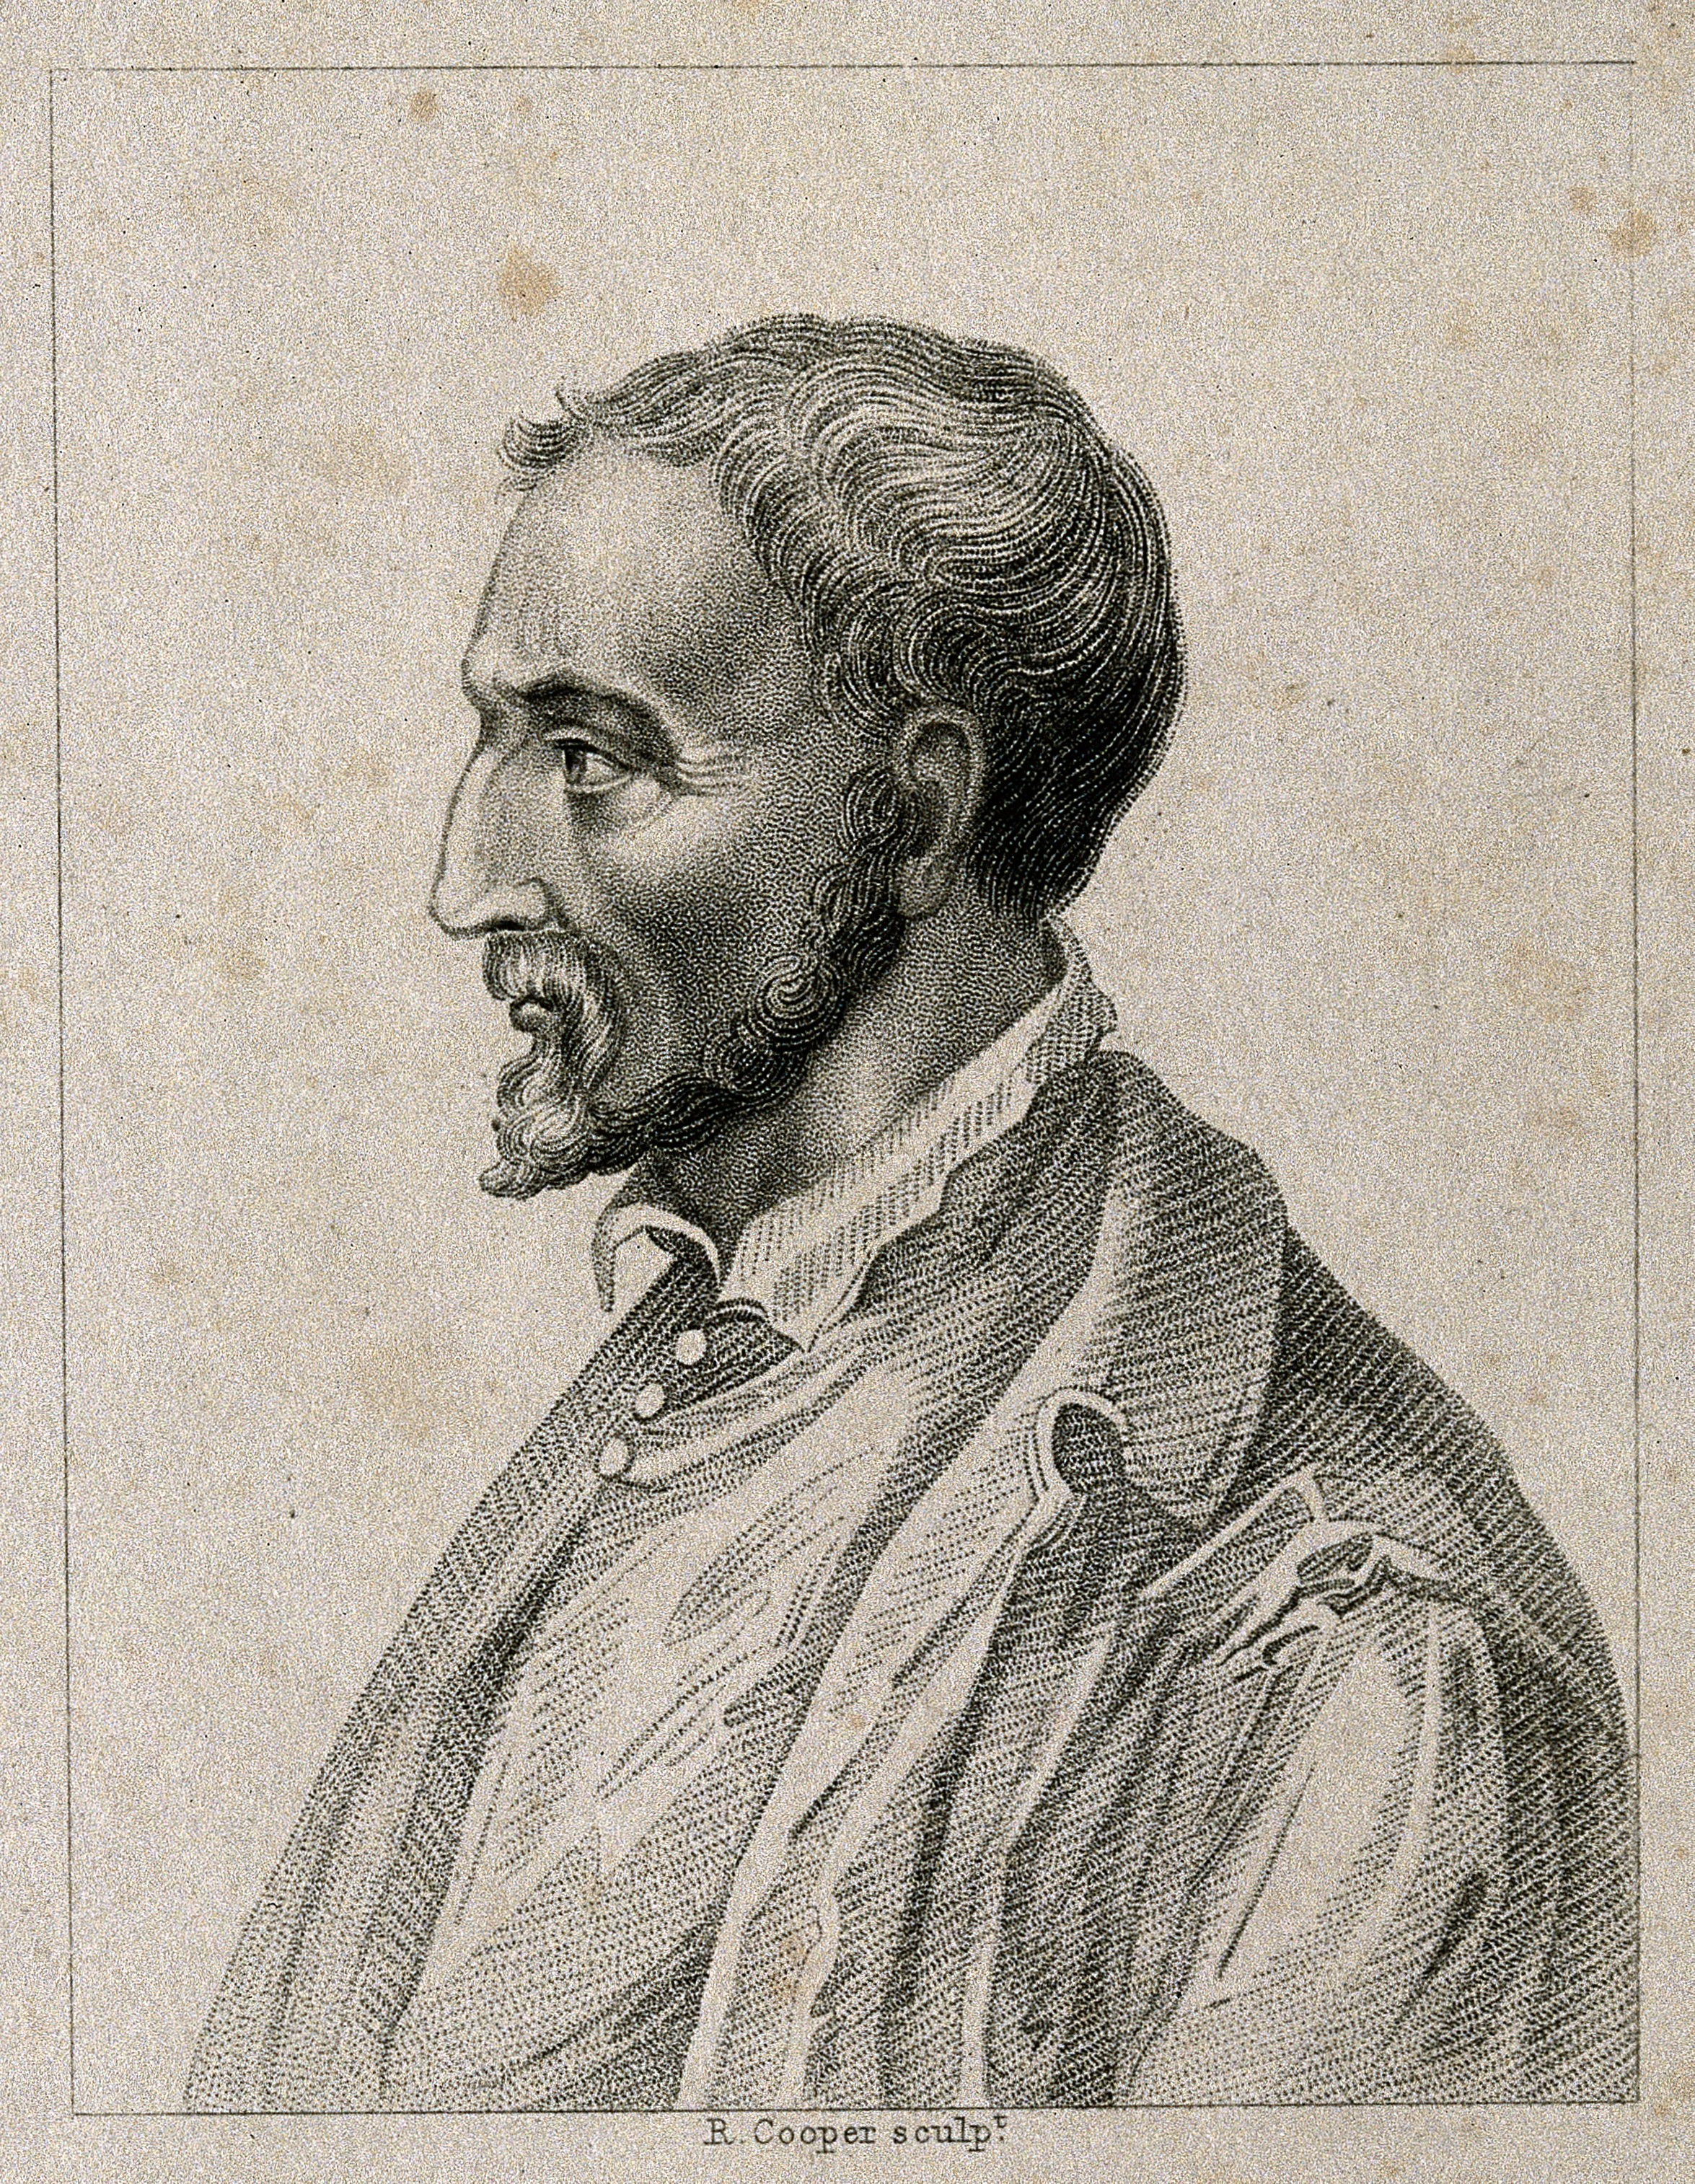
\includegraphics[width = 0.25\textwidth]{media/Girolamo_Cardano._Stipple_engraving_by_R._Cooper._Wellcome_V0001004.jpg}
    \caption{Holzstich aus dem 17. Jahrhundert von R. Cooper, der Cardano zeigen soll}
\end{center}
\end{figure}

Etwa hundert Jahre später (im Jahr 1624) erhielt die Wahrscheinlichkeitsrechnung einen weiteren Schub durch den Briefwechsel zweier grosser Mathematiker: Blaise Pascal  und Pierre de Fermat. Gegenstand des Briefwechsels waren wieder Fragen rund um Glücksspiele.

\begin{figure}[ht]
    \centering
    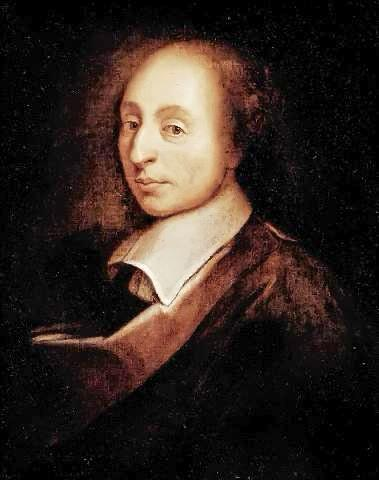
\includegraphics[width=0.25\textwidth]{media/Pascal_Blaise.jpeg}
    \hspace{1cm}
    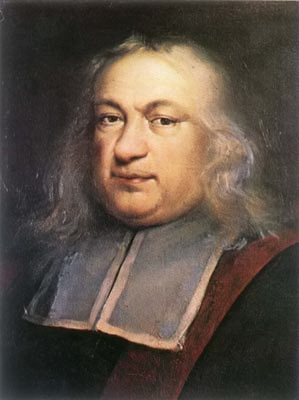
\includegraphics[width=0.25\textwidth]{media/Pierre_de_Fermat.jpg}
    \caption{Blaise Pascal (links) und Pierre de Fermat (rechts)}
\end{figure}

Allerdings beschränken sich die Anwendungen der Wahrscheinlichkeitsrechnung bei Weitem nicht aufs Glücksspiel. Schon im 17. Jahrhundert hat Christiaan Huygens, ein niederländischer Mathematiker, mit Hilfe von Wahrscheinlichkeiten berechnet, welche Witwenrente fair ist.

\begin{figure}[ht]
    \begin{center}
            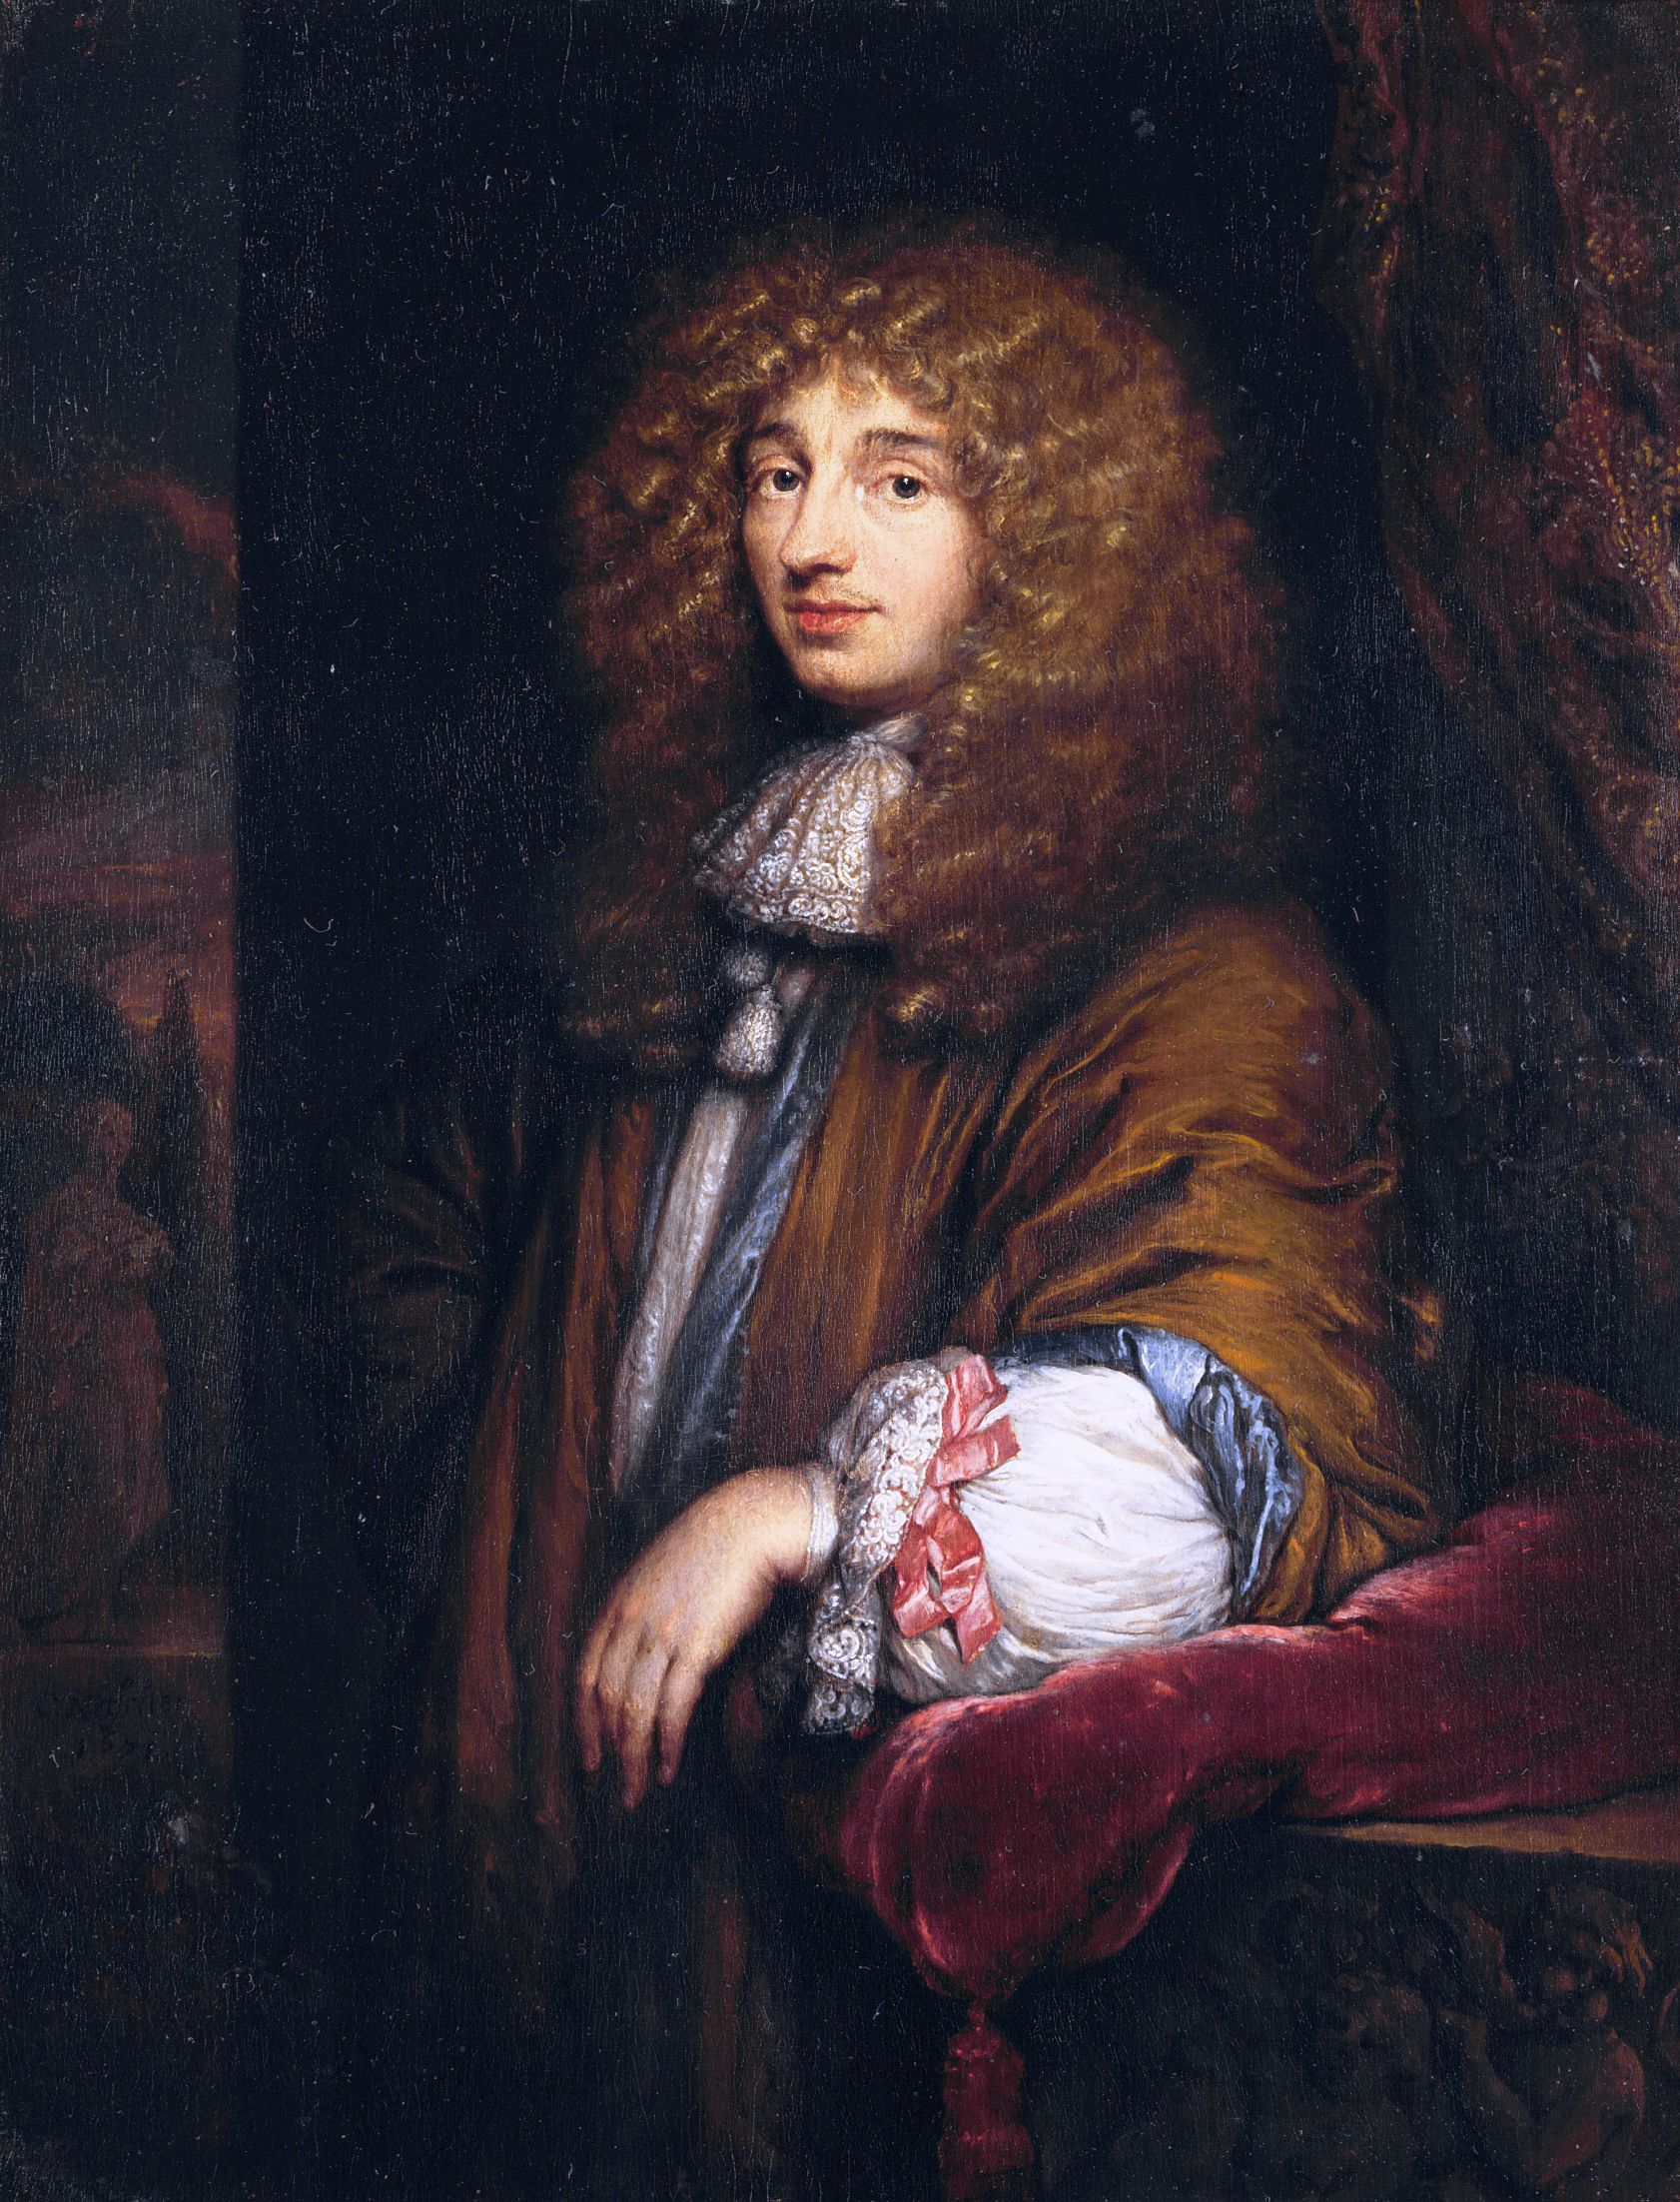
\includegraphics[width = 0.25\textwidth]{media/Christiaan_Huygens-painting.jpeg}
        \caption{Christiaan Huygens, 1671 von Caspar Netscher gemalt}
    \end{center}
    \end{figure}

Heute spielt die Wahrscheinlichkeitsrechnung in vielen Wissenschaften eine wichtige Rolle. Dazu gehören die Versicherungsbranche (Prämienberechnung) und die Finanzökonomie (Risikoanalyse). Ganz wichtig ist die Wahrscheinlichkeitsrechnung ausserdem in der Physik (Quantenmechanik), in allen Sozialwissenschaften (Auswerten von Statistiken) und in der Medizin (Sicherheit von Diagnose-Tests).








\clearpage
\subsection{Erste Begriffe und Laplace-Versuche}

Im Alltag spricht man oft von Wahrscheinlichkeiten, sodass wir bereits eine gute Vorstellung von diesem Begriff haben. Können Sie damit diese Fragen beantworten? 

\begin{LA}
{}{}
    \begin{enumerate}
        \item Ein Spielwürfel wird geworfen. 
        \begin{enumerate}
            \item Mit welcher Wahrscheinlichkeit erhält man eine 4?
            \item Mit welcher Wahrscheinlichkeit erhält man keine 4? 
            \item Was ist der Zusammenhang zwischen diesen beiden Wahrscheinlichkeiten?
        \end{enumerate}
        \item Beim Roulette sind die Felder mit den Zahlen 0, 1, 2, ..., 36 beschriftet.
        \begin{enumerate}
            \item Jemand setzt auf \textit{pair} – also darauf, dass der Ball auf eine gerade Zahl landet. Wie gross ist seine Gewinnwahrscheinlichkeit? (Beachte: 0 gehört nicht zu den geraden Zahlen)
            \item  Beim Roulette kann man auch auf das erste, zweite oder dritte Dutzend setzen. Wie gross ist die Gewinnwahrscheinlichkeit, wenn man auf das letzte Dutzend setzt (25 bis und mit 36)?
            \item Wie gross ist die Wahrscheinlichkeit, dass die Kugel auf einer Zahl landet, die gerade ist ODER zum letzten Dutzend gehört?
            \item Wie gross ist die Wahrscheinlichkeit, dass die Kugel auf einer Zahl landet, die gerade ist UND zum letzten Dutzend gehört?
        \end{enumerate}
        \item Ein roter und ein schwarzer Spielwürfel werden gleichzeitig geworfen. 
        \begin{enumerate}
            \item Welche Augensumme ist wahrscheinlicher: 11 oder 12?
            \item  Mit welcher Wahrscheinlichkeit zeigt mindestens einer der Würfel eine 6?
        
        \end{enumerate}
        
      
    \end{enumerate}
\end{LA}
\clearpage
Ein fairer Würfel wird geworfen. Dann ist die Wahrscheinlichkeit dafür, dass man eine Vier oder Fünf wirft $\frac{2}{6} = \frac{1}{3}$. Wir werden das so aufschreiben:
$$P(\text{Augenzahl 4 oder 5}) = \frac{1}{3}$$

Das `P' steht dabei abkürzend für `probabilitas' (Latein für Wahrscheinlichkeit). `Augenzahl 4 oder 5' ist hingegen ein `Ereignis':

\begin{definition}
    {Grundbegriffe der Wahrscheinlichkeit}{}
    \begin{itemize}
        \item  Ein Vorgang, der sich mindestens theoretisch beliebig oft wiederholen lässt und dessen Ergebnis nicht mit Sicherheit vorhergesagt werden kann, heisst \emph{Zufallsversuch}.
    
        \item Die Menge $S$ aller Ergebnisse eines Zufallsversuchs nennt man die \emph{Ergebnismenge} des Zufallsversuches.
        
        % \item  Eine Menge von Ergebnisse nennt man ein \emph{Ereignis}.
    
        \item Zufallsversuche, bei denen kein Grund ersichtlich ist, dass irgendeines der Ergebnisse eine grössere Chance hat aufzutreten, werden \emph{Laplace-Versuche}\footnote{Benannt nach dem französischen Mathematiker Pierre-Simon Laplace (1749-1827)} genannt.
    
        \item Wenn die Ergebnismenge eines Laplace-Versuchs $n$ Elemente beinhaltet, so ordnen wir jedem Element $s \in S$ die Wahrscheinlichkeit $p=\frac{1}{n}$ zu.
    
    \end{itemize}
   
\end{definition}

\begin{bsp}
{Laplace-Versuche}{}
Bei folgenden Zufallsversuchen scheint es berechtigt, von Laplace-Versuchen zu sprechen:

\begin{itemize}
    \item 	Münzwurf: Die Wahrscheinlichkeit für Kopf oder Zahl ist gleich: $P(K)=P(Z)= \frac{1}{2}$
    \item 	Würfeln: Jede Zahl hat die gleiche Chance: $P(1)=P(2)=\dots=P(6)=\frac{1}{6}$
    \item 	Roulette: Jedes Feld hat die gleiche Chance: $P(0)=P(1)=P(2)=\dots = P(36)=\frac{1}{37}$
\end{itemize}
\end{bsp}

Oft wird man mehrere Ergebnisse zusammen betrachten. In diesem Fall spricht man von \emph{Ereignissen}. Beim Roulette gehören zum Ereignis \emph{pair} die Ergebnisse $pair=\{2,4,6,\dots,32,34,36\}$

\begin{satz}
{Wahrscheinlichkeit bei Laplace-Versuchen}{}
Bei Laplace-Versuchen berechnet sich die Wahrscheinlichkeit \( P(E) \) eines Ereignisses \( E \) wie folgt:
\[
P(E) = \frac{\text{Anzahl zu } E \text{ gehörende Ergebnisse}}{\text{Anzahl aller möglichen Ergebnisse}}
\]
Oft spricht man kurz von „günstige Fälle / mögliche Fälle“:
\[
P(E) = \frac{\text{gF}}{\text{mF}}
\]
\end{satz}

\textbf{Vorsicht:} Man muss sorgfältig darauf achten, ob tatsächlich alle Ergebnisse die gleiche Chance haben. 
So glaubte der französische Mathematiker D’Alembert (1717–1783), dass beim gleichzeitigen 
Werfen von zwei Münzen die folgenden Ergebnisse gleichwahrscheinlich sind: 
Zweimal Wappen, einmal Wappen und einmal Zahl, zweimal Zahl.

Die richtige Rechnung zum Beispiel von D’Alembert lautet:

\[
\text{mF: WW, WZ, ZW, ZZ}
\]

\begin{itemize}
    \item Ereignis \( E_1 \) „zweimal Wappen“, \( \text{gF: WW} \quad P(E_1) = \frac{1}{4} \)
    \item Ereignis \( E_2 \) „zweimal Zahl“, \( \text{gF: ZZ} \quad P(E_2) = \frac{1}{4} \)
    \item Ereignis \( E_3 \) „einmal Wappen und einmal Zahl“, \( \text{gF: WZ oder ZW} \quad P(E_3) = \frac{1}{2} \)
\end{itemize}

\begin{ueb}
{}{}
\begin{enumerate}
    \item Augensumme beim Würfeln von zwei Spielwürfeln
    \begin{enumerate}
        \item Füllen Sie die Tabelle aus:
            \begin{center}
                
           
            \renewcommand{\arraystretch}{2} % Verdoppelt die Zeilenhöhe
            \setlength{\tabcolsep}{12pt}    % Passt den horizontalen Zellabstand an
            \begin{tabular}{|c|l|c|}
                \hline
                \textbf{Augensumme} & \textbf{Dazugehörige Ergebnisse} & \textbf{Wahrscheinlichkeit} \\
                \hline
                2  &                 &        \\
                \hline
                3  & (1,2) und (2,1) &        \\
                \hline
                4  &                 &        \\
                \hline
                5  &                 &        \\
                \hline
                6  &                 &        \\
                \hline
                7  &                 &        \\
                \hline
                8  &                 &        \\
                \hline
                9  &                 &        \\
                \hline
                10 &                 &        \\
                \hline
                11 &                 &        \\
                \hline
                12 &                 &        \\
                \hline
            \end{tabular}
        \end{center}
        
        \item 	Der deutsche Mathematiker Leibniz meinte, dass die Augensummen 11 und 12 beim gleichzeitigen Werfen von 2 Würfeln gleichwahrscheinlich sind. Worin bestand seine Fehlüberlegung?
    \end{enumerate}
    
        \item Bestimmen Sie die Wahrscheinlichkeit jedes Ereignisses.
        \begin{enumerate}
            \item Beim Wurf von zwei Münzen zeigen beide „Kopf“.
            \item Beim Wurf von drei verschiedenen Münzen zeigen genau zwei „Kopf“.
            \item Aus einer Urne mit drei gelben, vier grünen und acht blauen Kugeln wird eine gelbe Kugel gezogen.
            \item Aus der gleichen Urne (mit Vollbestand) ziehen Sie eine Kugel, die nicht blau ist.
        \end{enumerate}
        
        \item Wie gross ist die Wahrscheinlichkeit, mit zwei Laplace-Würfeln in einem Wurf:
        \begin{enumerate}
            \item die Summe 8 zu werfen,
        %     \item die Summe 9 zu werfen,
        %     \item die Differenz 2 zu werfen?
        % \end{enumerate}
        
        % \item Mit welcher Wahrscheinlichkeit erzielen Sie mit zwei Würfeln in einem Wurf:
        % \begin{enumerate}
            \item eine Summe von höchstens 5,
            \item die Differenz 2 zu werfen?
            \item eine Differenz von mindestens 3?
        \end{enumerate}
        
        \item Zwei Spieler werfen jeweils einmal einen homogenen Würfel. Wie gross ist die Wahrscheinlichkeit, dass die Augenzahlen verschieden sind?
        
        \item Zwei ideale Würfel werden gleichzeitig geworfen. Wie gross ist die Wahrscheinlichkeit, dass die grösste vorkommende Augenzahl höchstens 4 ist?
        
        \item Ein Glücksrad wird zweimal gedreht; die erste Drehung erzeugt die Zehnerziffer, die zweite die Einerziffer einer Zahl. Die zehn Kreissektoren sind gleich gross. Wie gross ist die Wahrscheinlichkeit:
        \begin{enumerate}
            \item für die Zahl 55,
            \item für die Quersumme 9,
            \item für eine Zahl zwischen 30 und 50 (ohne die beiden Grenzen)?
        \end{enumerate}
        \item Aus einer Urne mit 8 weissen, 6 blauen und mehreren roten Kugeln wird zufällig eine Kugel gezogen. Wie viele rote Kugeln sind in der Urne, wenn die Wahrscheinlichkeit:
        \begin{enumerate}
            \item dass die gezogene Kugel weiss ist, $\frac{2}{9}$ beträgt,
            \item dass die gezogene Kugel rot ist, $\frac{3}{5}$ beträgt,
            \item dass die gezogene Kugel blau ist, weniger als $\frac{2}{7}$ beträgt?
        \end{enumerate}
    
\end{enumerate}
\end{ueb}

\clearpage
Lösungen:

\begin{enumerate}
    \item Zu (b): Zur Erklärung ist es einfacher, wenn man einen Würfel rot und den anderen schwarz anmalt. Für die Augensumme zwölf müssen beide Würfel eine 6 zeigen. Für die Augensumme 11 gibt es hingegen zwei Möglichkeiten: Rot 5, schwarz 6 ODER rot 6, schwarz 5. 
    \item  
    \begin{enumerate}
        \item $\frac{1}{4}$
        \item $ \frac{3}{8} = 0.375$
        \item $ \frac{1}{5} = 0.2$
        \item$ \frac{7}{15} \approx 0.467$
    \end{enumerate}

    \item   \begin{enumerate}
        % \item $ \frac{1}{9}$
         \item $ \frac{5}{36}$
    %     \item $ \frac{2}{9} \approx 0.222$
    % \end{enumerate}

    % \item \begin{enumerate}
        \item $ \frac{5}{18} $
        \item $ \frac{2}{9} $
        \item $\frac{1}{3}$
    \end{enumerate}
    \item  $ \frac{5}{6} \approx 0.833$
    \item $ \frac{4}{9} \approx 0.444$
    \item \begin{enumerate}
        \item $\frac{1}{100}$
        \item $\frac{1}{10}$
        \item $\frac{19}{100}$
    \end{enumerate}
    \item Rote Kugeln:
    \begin{enumerate}
        \item$22$ rote Kugeln
        \item $21$ rote Kugeln
        \item mindestens $8$ rote Kugeln
    \end{enumerate}
    
\end{enumerate}
\pagebreak





\subsection{Wahrscheinlichkeiten und relative Häufigkeit}
\begin{LA}
    {}{}
    \begin{enumerate}
        \item Die Wahrscheinlichkeit für eine Null im Roulette beträgt $\frac{1}{37}$. Angenommen an einem Tag wird das Roulette-Rad 400-mal gedreht. Ungefähr wie häufig wird die Kugel bei der Null stehenbleiben?
        \item Bei der Berechnung der Prämie einer Todesfallversicherung muss das Versicherungsunternehmen abschätzen, wie gross die Wahrscheinlichkeit ist, dass der Versicherungsnehmer in einer bestimmten Zeitspanne (z.B. 10 Jahre) sterben wird. Was denken Sie: Wie wird diese Wahrscheinlichkeit geschätzt?
    \end{enumerate}
\end{LA}
\pagebreak
Bisher wurde stets von der Laplace-Vermutung ausgegangen, also davon, dass alle Ergebnisse die gleiche Chance haben einzutreffen. Es stellten sich zwei Fragen
\begin{itemize}
    \item Wie man prüfen kann, ob die Laplace-Vermutung berechtigt ist?
    \item Wie kann man die Wahrscheinlichkeit für Ereignisse schätzen, wenn die Ergebnisse nicht alle gleichwahrscheinlich sind?
\end{itemize}

Beide Fragen lassen sich beantworten, indem man die relative Häufigkeit des Eintreffen eines Ereignisses untersucht.

Dazu wird der Versuch mehrere Male durchgeführt. Die Häufigkeit des Auftretens eines Ergebnisses wird dann mit der Anzahl Versuche (= Stichprobenumfang) verglichen.

\begin{bsp}{Häufigkeit von 6 beim Würfeln}{}
    Ein Würfel wird mehrmals geworfen. Dabei wird gezählt, wie häufig das Ereignis $E:$ `Augenzahl 6' eintritt.
    \smallskip

        \centering \footnotesize
        \begin{tabular}{|c|c|c|c|c|c|c|c|c|c|c|}
        \hline
        \textbf{Anzahl Würfe} $n$ & 40 & 80 & 120 & 160 & 200 & 240 & 280 & 320 & 360 & 400 \\ \hline
        \vtop{\hbox{\strut \textbf{Absolute}}\hbox{\strut \textbf{Häufigkeit} $k$}} & 6 & 10 & 17 & 21 & 29 & 40 & 50 & 56 & 60 & 65 \\ \hline
        \vtop{\hbox{\strut \textbf{Relative}}\hbox{\strut \textbf{Häufigkeit} $k/n$}} & 0.150 & 0.125 & 0.142 & 0.131 & 0.145 & 0.167 & 0.179 & 0.175 & 0.167 & 0.163 \\ \hline
        \end{tabular}
    
        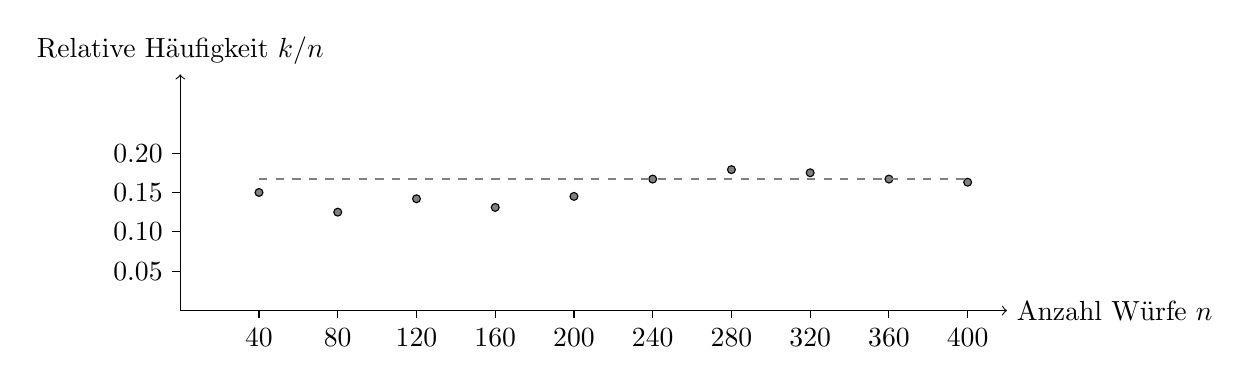
\begin{tikzpicture}
            % Achsen
            \draw[->] (0,0) -- (10.5,0) node[right] {Anzahl Würfe \(n\)};
            \draw[->] (0,0) -- (0,3) node[above] {Relative Häufigkeit \(k/n\)};
            
            % Beschriftungen der x-Achse
            \foreach \x/\label in {1/40, 2/80, 3/120, 4/160, 5/200, 6/240, 7/280, 8/320, 9/360, 10/400} {
                \draw (\x,0) -- (\x,-0.1) node[below] {\label};
            }
        
            % Beschriftungen der y-Achse
            \foreach \y/\label in {0.5/0.05, 1/0.10, 1.5/0.15, 2/0.20} {
                \draw (0,\y) -- (-0.1,\y) node[left] {\label};
            }
            
            % Datenpunkte
            \foreach \x/\y in {1/1.5, 2/1.25, 3/1.42, 4/1.31, 5/1.45, 6/1.67, 7/1.79, 8/1.75, 9/1.67, 10/1.63} {
                \draw[fill=gray] (\x,\y) circle (0.05);
            }
            
            % Linie
            \draw[thick, gray, dashed] (1,1.666) --  (10,1.666);
       
        \end{tikzpicture}
    
        
\end{bsp}

\begin{satz}
    {Das Gesetz der grossen Zahlen}{}
    Bei langen Versuchsreihen stabilisieren sich die relativen Häufigkeiten eines Ergebnisses in der Nähe der Wahrscheinlichkeit des Ergebnisses.
\end{satz}

Mit diesem Gesetz ist es auch möglich, Wahrscheinlichkeiten von Ergebnissen von nicht-Laplace-Versuchen zu schätzen.

Ein Beispiel für diese Art der Schätzung von Wahrscheinlichkeiten findet Anwendung in der Lebensversicherung: Beim Abschliessen einer Todesfallversicherung bestimmt man eine Vertragsdauer und einen Versicherungsbetrag. Wenn die versicherte Person am Ende der Vertragsdauer noch lebt, wird ihr der vereinbarte Versicherungsbetrag ausbezahlt.

Wie teuer soll so eine Versicherung sein? Um das zu bestimmen, benötigt man eine Schätzung der Wahrscheinlichkeit, dass die versicherte Person während der Vertragsdauer stirbt. Dazu werden die sogenannten `Sterbetafeln' studiert.

\begin{figure}[ht]
    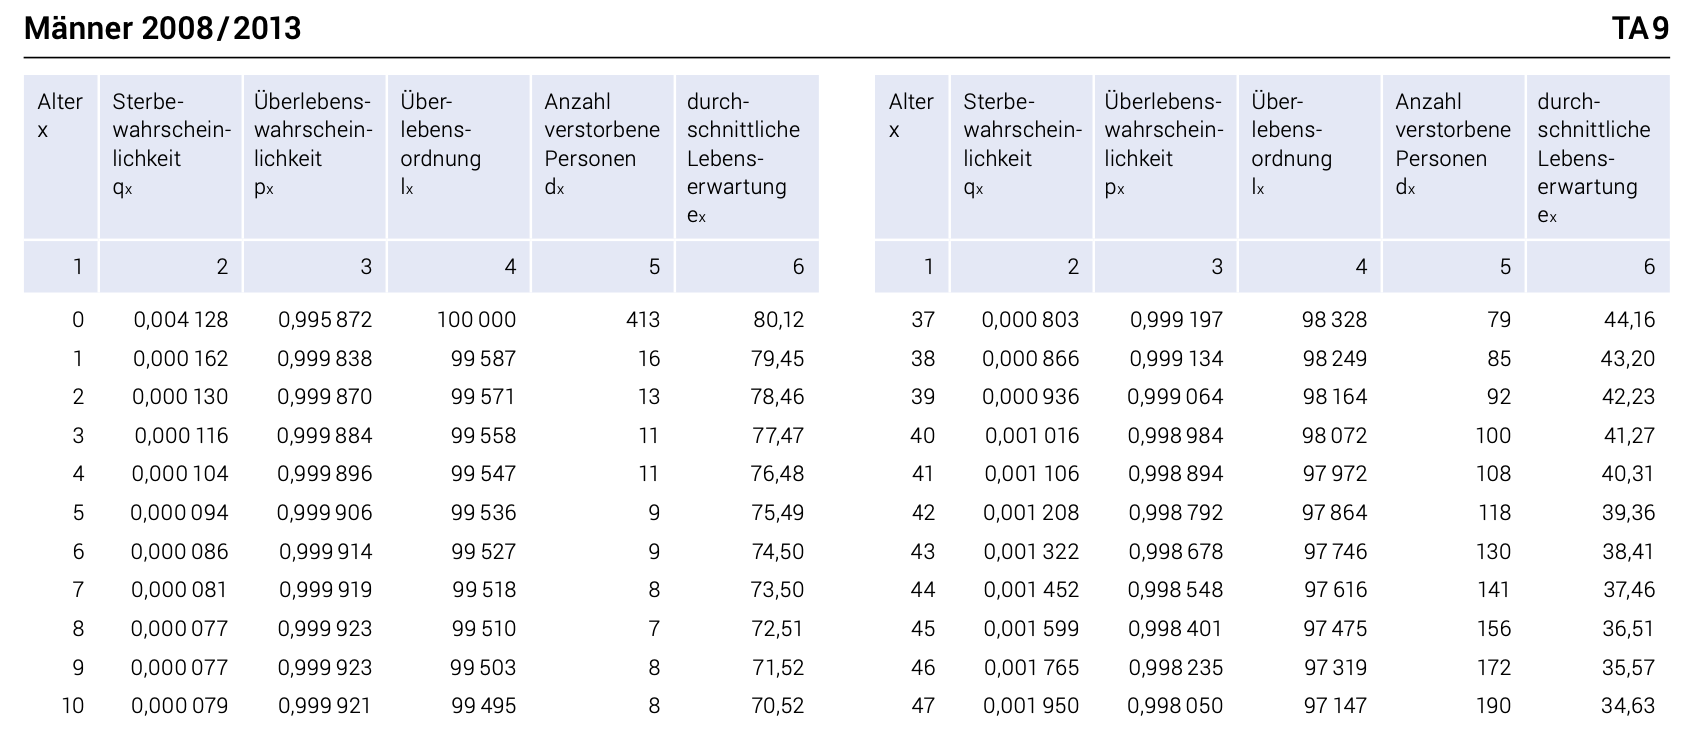
\includegraphics[width = 0.9 \textwidth]{media/Sterbetafel.png}
    \caption{Auszug aus  `Sterbetafeln für die Schweiz 2008-2013', \href{https://www.bfs.admin.ch/bfs/de/home/statistiken/kataloge-datenbanken.assetdetail.2103067.html}{BFS}}
    \label{fig:Sterbetafel}
\end{figure}

\begin{bsp}
{10 Jahre Überlebenswahrscheinlichkeit eines 37-Jährigen}{}
(Wird im Unterricht ergänzt)
\vspace*{5cm}
\end{bsp}

% So einfach und plausibel das Gesetz der grossen Zahlen klingt, so häufig wird es doch falsch gedeutet. Das betrifft besonders die Situation, bei der innerhalb einer begonnenen Versuchsreihe ein Ereignis im Vergleich zu seiner Wahrscheinlichkeit über- oder unterrepräsentiert ist. Wie ist es möglich, dass sich ein solches Ungleichgewicht wieder ausgleicht, wie es das Gesetz der grossen Zahlen vorhersagt? Es liegt nahe zu erwarten, dass dazu ein gegenläufiger Ausgleich nötig ist. Aber muss es wirklich ein gegenläufiger Ausgleich sein? Das heisst, kann beim Roulette ein voruebergehendes Übergewicht roter Zahlen nur dadurch ausgeglichen werden, dass danach weniger rote Zahlen erscheinen, als es der Wahrscheinlichkeit eigentlich entspricht?

% Nehmen wir als Beispiel Roulette-Sequenzen von je 37 Spielen, in denen sich aufgrund des Gesetzes der grossen Zahlen durchschnittlich 18-mal „Rot“ ergibt. Werden in der ersten Sequenz 25 rote Zahlen ausgespielt, dann ist „Rot“ gegenueber dem theoretischen Durchschnitt mit 7 Treffern im Übergewicht. Bei 23 roten Zahlen in der zweiten 37er-Sequenz verstärkt sich das Übergewicht sogar noch auf \(7+5=12\) rote Zahlen. Ein gegenläufiger Ausgleich hat also nicht stattgefunden. Trotzdem hat sich die relative Häufigkeit der Wahrscheinlichkeit von \(18/37\) angenähert, nämlich von \(25/37 \) auf  \( (25 + 23)/(2\cdot37) =  24/37\).






\clearpage
\subsection{Die Sätze der Wahrscheinlichkeitsrechnung}

\begin{LA}
{}{}

Ein roter und ein grüner Würfel werden geworfen. Welche Wahrscheinlichkeiten haben die folgenden Ereignisse:

\begin{enumerate}
    \item \textbf{Ereignis $A$:} Der rote Würfel zeigt eine 6.
    \item \textbf{Ereignis $B$:} Der grüne Würfel zeigt eine 6.
    \item \textbf{Und-Ereignis \(A \cap B\):} Beide Würfel zeigen eine 6.
    \item \textbf{Oder-Ereignis \(A \cup B\):} Der rote oder der grüne Würfel zeigt eine 6.
    \item \textbf{Gegenereignis \(\bar{A}\):} Der rote Würfel zeigt keine 6.
    \item Bob berechnet die Wahrscheinlichkeit für das Ereignis \(A \cup B\) (Der rote oder der grüne Würfel zeigt eine 6) so:

    \[
    1 - \left(\frac{5}{6}\right)^2 = \frac{11}{36}
    \]
    
    Erklären Sie, welche Überlegung hinter dieser Rechnung steht.
\end{enumerate}

\end{LA}
\pagebreak

\begin{definition}
    {Sichere, Unmögliche, Gegen-, Und-, Oder-Ereignisse}{}

Sei \(S\) der Ergebnisraum eines Zufallsexperiments und seien \(A, B \subseteq S\) Ereignisse:

\begin{itemize}
    \item \(P(S) = 1\): Das \emph{sichere Ereignis} hat die Wahrscheinlichkeit 1.
    \item \(P(\emptyset) = 0\): Das \emph{unmögliche Ereignis} hat die Wahrscheinlichkeit 0.


\item Die Wahrscheinlichkeit, dass \(A\) nicht eintritt, ist:

\[
P(S \setminus A) = P(\bar{A}) = 1 - P(A)
\]

\( \bar{A} \) nennt man auch \emph{Gegenereignis}.

\item  Sind zwei Ereignisse \(A\) und \(B\) unabhängig\footnote{Tatsächlich ist es nicht immer einfach festzustellen, ob zwei Ereignisse unabhängig sind. Darauf gehen wir aber vorerst noch nicht ein.} voneinander, so ist die Wahrscheinlichkeit, dass \(A\) und \(B\) eintreffen:

\[
P(A \cap B) = P(A) \cdot P(B)
\]

\item Die Wahrscheinlichkeit, dass \(A\) oder \(B\) eintritt, ist:

\[
P(A \cup B) = P(A) + P(B) - P(A \cap B)
\]

\end{itemize}
\end{definition}

Das Betrachten des Gegen-Ereignisses kann die Rechnungen manchmal erheblich vereinfachen:

\begin{bsp}
    {Wahrscheinlichkeit für keine 6}{}

Vier Würfel werden geworfen. Wie gross ist die Wahrscheinlichkeit für das Ereignis \(A\): mindestens eine Sechs erscheint?

In diesem Fall lohnt es sich, das Gegenereignis zu betrachten: \(\bar{A}\): keine Sechs erscheint.

\[
P(\text{mindestens 1x6}) = 1 - P(\text{keine 6})
\]

Die Wahrscheinlichkeit, dass der erste Würfel keine 6 zeigt, ist \(\frac{5}{6}\). Das gleiche gilt für jeden weiteren Würfel. Da die Würfel unabhängig sind, ist die Wahrscheinlichkeit, dass der erste keine 6 \textbf{UND} der zweite keine 6 \textbf{UND} der dritte keine 6 \textbf{UND} der vierte keine 6 zeigt:

\[
P(\text{keine 6}) = \frac{5}{6} \cdot \frac{5}{6} \cdot \frac{5}{6} \cdot \frac{5}{6} = \left(\frac{5}{6}\right)^4
\]

Also:

\[
P(\text{mindestens 1x6}) = 1 - \left(\frac{5}{6}\right)^4 \approx 51{,}8\,\%
\]

\end{bsp}

\begin{satz}
    {Merksatz}{}
    Bei Aufgaben mit einem „mindestens“ bzw. „höchstens“ sollte man prüfen, ob nicht der Über-gang zur Wahrscheinlichkeit des Gegen-Ereignisses vorteilhaft ist.
\end{satz}

\begin{ueb}
    {}{}
    \begin{enumerate}
        \item Aus einem deutschschweizer Jasskartenspiel mit 36 Karten wird eine Karte gezogen.
        \begin{enumerate}
            \item Wie gross ist die Wahrscheinlichkeit, dass es sich dabei um eine Rosenkarte handelt?
            \item Wie gross ist die Wahrscheinlichkeit, dass es sich dabei nicht um eine Rosenkarte handelt?
            \item Wie ändern sich die Wahrscheinlichkeiten in a) und b), wenn Sie bereits zwei Rosenkarten und vier Schellenkarten auf der Hand halten?
        \end{enumerate}
    
        \item Nehmen Sie an, dass von den 400'000 Einwohnern in Zürich 25'000 reich sind, 2'000 berühmt, davon sind 1'500 sowohl reich als auch berühmt. Es wird zufällig ein Einwohner von Zürich aus dem Einwohnerregister ausgewählt.
        \begin{enumerate}
            \item Wie wahrscheinlich ist es, dass die gewählte Person nicht berühmt ist?
            \item Wie wahrscheinlich ist es, dass die gewählte Person weder reich noch berühmt ist?
            \item Wie wahrscheinlich ist es, dass die gewählte Person berühmt, aber nicht reich ist?
        \end{enumerate}
    
        \item Sie würfeln zweimal nacheinander. Beschreiben Sie jeweils das Gegenereignis und berechnen Sie dessen Wahrscheinlichkeit.
        \begin{enumerate}
            \item Sie werfen mindestens einmal eine Fünf.
            \item Sie werfen höchstens einmal eine Fünf.
            \item Sie werfen genau einmal eine Fünf.
        \end{enumerate}
    
        \item Gehen Sie in dieser Aufgabe davon aus, dass die Wahrscheinlichkeit für einen Geburtstag an jedem Tag des Kalenderjahres gleich ist (Gleichverteilung). Den 29. Februar können Sie dabei vernachlässigen.
        \begin{enumerate}
            \item Wie gross ist die Wahrscheinlichkeit, dass zwei zufällig gewählte Personen nicht am gleichen Tag Geburtstag haben?
            \item Wie gross ist die Wahrscheinlichkeit, dass zwei zufällig gewählte Personen am gleichen Tag Geburtstag haben?
            \item Wie gross ist die Wahrscheinlichkeit, dass in einer Gruppe von vier Personen alle an verschiedenen Tagen Geburtstag haben?
            \item Formulieren Sie das Gegenereignis von c) und berechnen Sie dessen Wahrscheinlichkeit.
            \item Wie viele Personen müssen in einer Gruppe sein, damit die Wahrscheinlichkeit, dass es in der Gruppe mindestens zwei Personen gibt, welche am gleichen Tag Geburtstag haben, über 50\% liegt? 
            \item Ist die Annahme einer Gleichverteilung gerechtfertigt? Wie könnte man das überprüfen?
        \end{enumerate}
    
    \end{enumerate}
\end{ueb}

\clearpage
Lösungen:
\begin{enumerate}
  
        \item
        \begin{enumerate}
            \item \(\frac{1}{4}\)
            \item \(\frac{3}{4}\)
            \item \(\frac{7}{30}, \frac{23}{30}\)
        \end{enumerate}
       
        \item
        \begin{enumerate}
            \item \(\frac{199}{200}\)
            \item \(\frac{749}{800}\)
            \item \(\frac{1}{800}\)
        \end{enumerate}
        \item
        \begin{enumerate}
            \item \(\frac{25}{36}\)
            \item \(\frac{1}{36}\)
            \item \(\frac{13}{18}\)
       
    \end{enumerate}
    \item
\begin{enumerate}
    \item \(\frac{364}{365}\)
    \item \(\frac{1}{365}\)
    \item \(98.4\%\)
    \item \(1.6\%\)
    \item \(n \geq 23\) Mit Pröbeln oder mit einem kleinen Python-Programm:
    \lstinputlisting[language=Python]{media/Geburtstagsparadoxon.py}
    \item \(-\)
\end{enumerate}
\end{enumerate}